% AdvancedNetworks_29-03-2013.tex - Assignment for Computer Networks

\documentclass[9pt, a4paper, oneside]{article}

\usepackage[english]{babel}
\usepackage{multicol}
\usepackage[a4paper]{geometry}
\usepackage[firstpage=true,
    vshift=-2cm,
        hshift=-5cm]
                {background}

\backgroundsetup{contents={
        \begin{minipage}[b]{50mm}
            \centering
                Prof. Danny Hughes \\
                    \texttt{danny.hughes@cs.kuleuven.be}
        \end{minipage}
}}
\SetBgScale{1}
\SetBgColor{black}
\SetBgAngle{0}
\SetBgOpacity{1}
\SetBgPosition{current page.north east}

\begin{document}

\title{Computer Networks: Advanced Networks}
\author{Toon Nolten r0258654\\
    \texttt{toon.nolten@student.kuleuven.be}
        }
\date{\today}
\maketitle

\newpage

\section{Reference Models}

\subsection{Compare and contrast the OSI and TCP/IP reference models.}

The OSI model was conceived as a model, there were no protocols that needed to
fit the model. The TCP/IP model on the other hand was made to fit the existing
TCP/IP protocols. As a consequence the TCP/IP model fits perfectly
with the TCP/IP protocols but not at all with other protocols, so the model
is of little use and the OSI model was made without experience in designing
protocols, so some protocols can't fit the model and some model concepts are
of little use (presentation and session layers).

\subsection{Map the following protocols to the OSI stack}

\begin{center}
\begin{tabular}{l | l}
    OSI Layer & Protocol \\
    \hline
    Application & BitTorent, HTTP, FTP \\
    Presentation &  \\
    Session & SSL \\
    Transport & TCP, UDP \\
    Network & IPv4, IPv6 \\
    Data link & Ethernet, 802.11g \\
    Physical &  \\
\end{tabular}
\end{center}

\subsection{Discuss, with reference to specific protocols the problem of
            ambiguity when mapping protocols to the OSI stack}

\begin{multicols}{2}
\begin{description}
    \item[SSL] \hfill \\
        SSL fits in the application layer as an application that encrypts your
        network traffic.
        But it also fits in the session layer because it provides a secure
        session.
        One could also argue for the presentation layer, you use encryption
        to represent your data.
    \item[RTP] \hfill \\
        RTP makes use of UDP for transmission and is implemented in user space,
        therefore it fits in the application layer.
        However, RTP offers a generic transport service (realtime transport),
        so it also fits in the transport layer.
    \item[DHCP] \hfill \\
        DHCP is an application that makes use of UDP broadcast, which means
        it fits in the application layer.
        But DHCP is used to acquire an IP address which is a network layer
        level address, so it could also be put in the network layer.
    \item[ARP] \hfill \\
        ARP resolves network layer addresses into link layer address.
        It fits in the network layer because it makes use of the link layer,
        it fits in the link layer because that's where it is used (to turn a
        network level address into a link level address).
    \item[DNS] \hfill \\
        DNS is placed in the application layer because it makes use of UDP.
        But it uses information about network layer addresses so it fits in
        the network layer.
    \item[TCP] \hfill \\
        TCP more or less fits in the network layer.
        However the network layer is best-effort and implemented throughout
        the network (in routers) so an extra layer is needed that ensures
        reliable transport and is completely controlled by your host.
\end{description}
\end{multicols}

\section{Connection Establishment}

\subsection{Describe how the relationship between initial sequence numbers and
            time arises}

To make sure that there is no window overlap after a crash we need a new
sequence number to start our sliding window from, that is not in use anymore.
To acquire such a number we need a realtime clock that keeps ticking during
a crash, we can then take the lower-order bits of the clock as our new initial
sequence number.
This means the clock must advance slow enough not to wrap around during the
crash.

\subsection{Describe what the \emph{forbidden region} of sequence numbers is
            and why this region exists}

Any segment with a sequence number in the \emph{forbidden region} should be
discarded.
This is because a segment with a \emph{forbidden} sequence number could be
a delayed segment.

\subsection{Describe the limitations necessary to ensure that sequence numbers
            do not enter the \emph{forbidden region}}

There are two ways a host could enter the \emph{forbidden region}, generating
sequence numbers too fast or too slow with regard to the realtime clock.
If sequence numbers are generated too fast the numbers can catch up with the
\emph{forbidden region} of segments that are still alive in the network.
If sequence numbers are generated too slow, the \emph{forbidden region}
catches up with the sequence numbers you're using.

\subsection{Demonstrate using a graph, the two ways in which a host could
            enter the \emph{forbidden region}}

\begin{figure}[h]
\centering
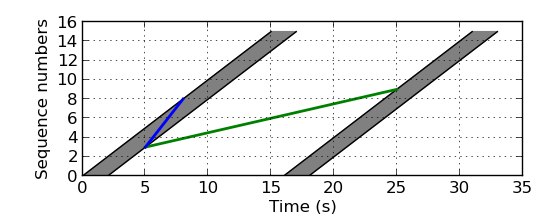
\includegraphics{forbiddenregion.png}
\caption{Entering the forbidden region}
\end{figure}

\newpage

\section{Congestion}

\subsection{Define the concepts of \emph{Convergence} and \emph{Oscillation}.
            What causes oscillation to occur?}

Convergence is when the allocation of bandwidth stops changing.
This allocation should ideally be fair and efficient.
Oscillation is a repeated over- and underadjustment around the ideal point of
convergence.
Oscillation occurs when the adjustment of bandwidth allocation is too fast,
which causes overshoot and succesive underadjustment, etc.

\subsection{Describe the principles of the Additive Increase Multiplicative
            Decrease approach}

Convergence can only be achieved if the rate of increase and decrease are not
equal.
Since congestion should be avoided at all cost, AIMD uses additive (slow)
increase and multiplicative (fast) decrease.
Because an increase in bandwidth is done additively it can take a long time
after starting, to reach a reasonable bandwidth.
To speed this up \emph{slow start} was introduced, this increases bandwidth
exponentially instead of additively, so it's much faster.

\subsection{Demonstrate using a graph the convergence of AIMD towards the
            Optimal bandwidth allocation for two transport elements with
            equal performance transport layer connections.}

\begin{figure}[h]
\centering
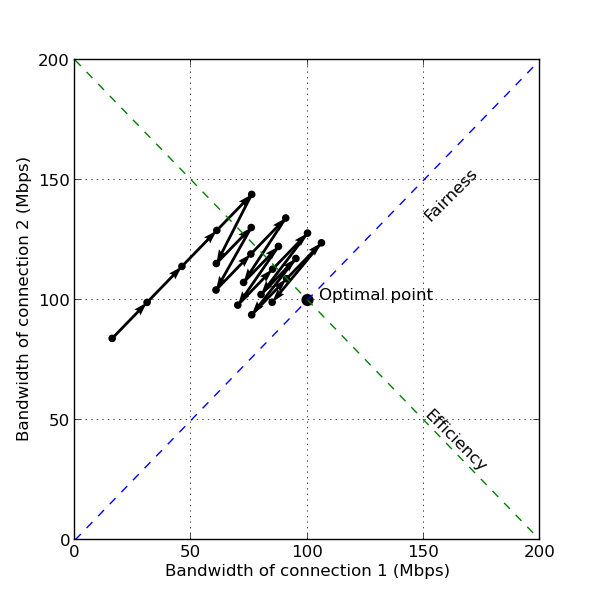
\includegraphics[scale=0.6]{aimd.png}
\caption{Additive Increase Multiplicative Decrease}
\end{figure}

\end{document}
